\documentclass{beamer}
\usepackage[english]{babel} %%remove tildes e.q. in bibliography
\usepackage{nicefrac}
\usepackage{graphicx}
\usepackage{url}
\usepackage{natbib}
\usepackage{bibentry}
\bibliographystyle{apalike}
\usepackage{chngcntr}
\counterwithin*{footnote}{page}
\newcommand\footcite[1]{\footnote{\tiny{\bibentry{#1}}}\label{\thepage:#1}}
\newcommand\secondcite[1]{\textsuperscript{\ref{\thepage:#1}}}

\setbeamertemplate{caption}[numbered]
\setbeamertemplate{navigation symbols}{}

% \def\newblock{\hskip .11em plus .33em minus .07em}
% \newcommand{\newblock}{}

\newcommand{\software}[1]{\textsl{#1}}
\newcommand\R{\software{R}}
% 
\newcommand\Bioconductor{\software{Bioconductor}}
\newcommand{\Rpackage}[1]{{\usebeamercolor[fg]{structure} \textsl{#1}}}
\newcommand\Biocpkg[1]{%
  {\href{http://bioconductor.org/packages/release/bioc/html/#1.html}%
    {\Rpackage{#1}}}}
\newcommand\Biocannopkg[1]{%
  {\href{http://bioconductor.org/packages/release/data/annotation/html/#1.html}%
    {\Rpackage{#1}}}}
\newcommand\Biocexptpkg[1]{%
  {\href{http://bioconductor.org/packages/release/data/experiment/html/#1.html}%
    {\Rpackage{#1}}}}
\newcommand\CRANpkg[1]{%
  {\href{http://cran.fhcrc.org/web/packages/#1/index.html}%
    {\Rpackage{#1}}}}
% 

\newcommand{\Robject}[1]{{\texttt{#1}}}
\newcommand{\Rfunction}[1]{{\texttt{#1}}}
\newcommand{\Rclass}[1]{\textit{#1}}
\newcommand{\Rexpression}[1]{\texttt{#1}}
\newcommand{\Rmethod}[1]{{\texttt{#1}}}
\newcommand{\Rfunarg}[1]{{\texttt{#1}}}

\title{Removing batch-effects from expression data}
\author{Maarten van Iterson}
\institute[LUMC]{\\Leiden University Medical Center\\Department of Molecular Epidemiology}
\date{\today}

\newenvironment{wideitemize}{\itemize\addtolength{\itemsep}{0.2in}}{\enditemize}

\setbeamertemplate{itemize item}{-}
\setbeamertemplate{itemize subitem}{-}
\setbeamertemplate{itemize subsubitem}{-}

\begin{document}

\nobibliography{batch}

\frame{\titlepage}

\begin{frame}
  \frametitle{Batch-Effects}
  \begin{quote}
    In differential expression analyses there are primary variables of interest and often other nuisance factors, technical or biological, that introduce unwanted variation.
  \end{quote}
  \pause
  \begin{wideitemize}
  \item biological nuisance factors:
    \begin{itemize}
    \item gender, age, white blood cell composition, etc.
    \end{itemize}
    \pause
  \item technical nuisance factors (batch effects):
    \begin{itemize}
    \item lab, sequence machine, library generation date, operator, etc.
    \end{itemize}
    \pause
  \item Often not all factors are known!
  \end{wideitemize}
  \pause
  \textbf{Confounding} occurs when there is correlation between primary variable of interest and the outcome
\end{frame}

\begin{frame}
  \frametitle{GEUVADIS RNAseq data\footcite{Hoen2013}}
  \begin{figure}
    \centering
    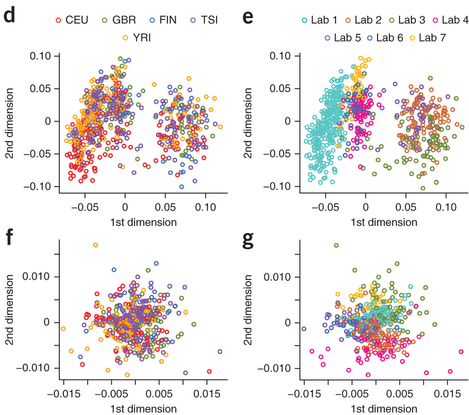
\includegraphics[width=0.6\textwidth]{geuvadis}
    \caption{(d) MDS plot of RNAseq data before batch correction colored by population and (e) colored by laboratory, (f) after batch correction colored by population and (e) colored by laboratory.}
  \end{figure}
\end{frame}

\begin{frame}
  \frametitle{Batch correction methods}
  \begin{wideitemize}
  \item normalization methods:
    \begin{itemize}
    \item quantile normalization, trimmed mean of M-values (TMM) \Biocpkg{edgeR}
    \end{itemize}
    \pause
  \item technology specific:
    \begin{itemize}
    \item within-plate-, print-tip-normalization, etc.
    \item GC-bias correction methods \Biocpkg{cqn}\footcite{Hansen2012}, \Biocpkg{EDASeq}\footcite{Risso2011}
    \end{itemize}
    \pause
  \item Batch correction methods:
    \begin{itemize}
    \item \textbf{Nuisance factors are known}: linear model, ComBat
    \item \textbf{Nuisance factors are unknown}: estimate batch-effects from the data
      \begin{itemize}
      \item controls e.g. spike-ins or housekeeping
      \item principal components
      \item $\cdots$
      \end{itemize}
    \end{itemize}
  \end{wideitemize}
\end{frame}

\begin{frame}
  \frametitle{Normalization does not remove batch-effects}
  \begin{figure}
    \centering
    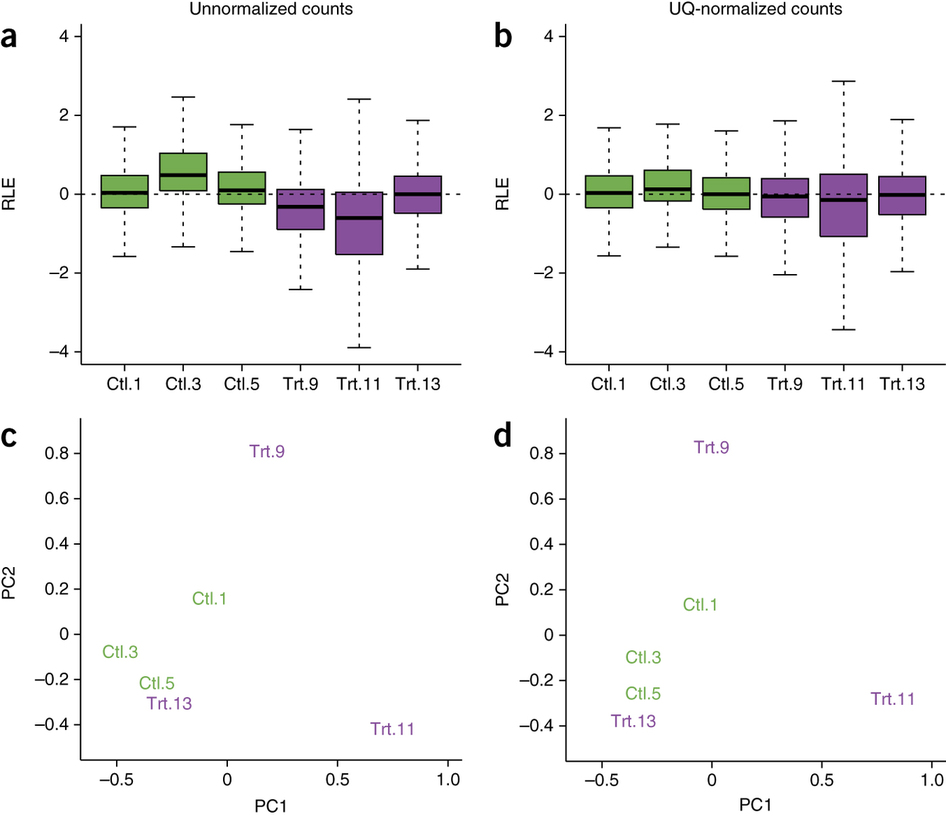
\includegraphics[width=0.55\textwidth]{risso1.jpg}
    \caption{Raw vs upper-quartile-normalized data \footcite{Risso2014}}
  \end{figure}
\end{frame}

\begin{frame}
  \frametitle{Removing batch-effects using RUV}
  \begin{figure}
    \centering
    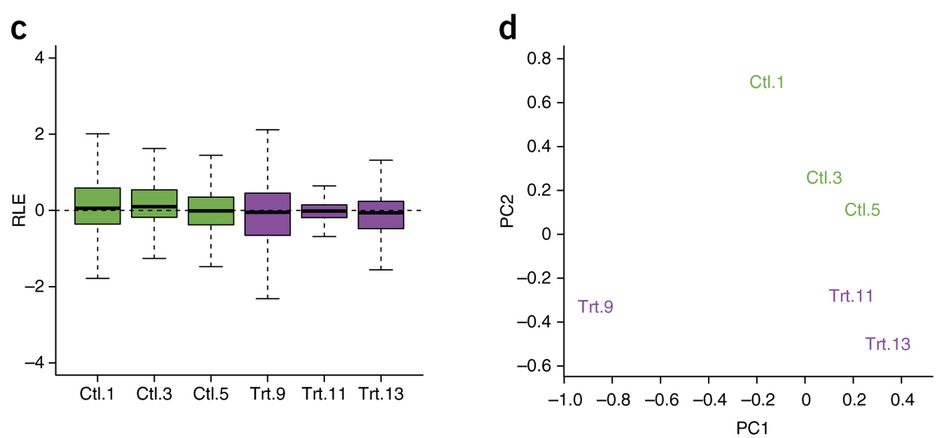
\includegraphics[width=0.85\textwidth]{risso2cd.jpg}
    \caption{RUV estimate and corrected}
  \end{figure}
\end{frame}

\begin{frame}
  \frametitle{ComBat\footcite{Johnson2007}}
  Usage:
  \begin{itemize}
  \item Input: Known batches
  \item Output: Batch corrected expression matrix
  \end{itemize}
  \pause
  Method briefly:
  \begin{itemize}
  \item Mean center and standardize the variance of each batch for each gene independently
  \item Use an empirical Bayes approach to estimate robust mean and variance
  \end{itemize}
  \pause
  Remarks:
  \begin{itemize}
  \item Specially suited for small sample microarray studies
  \item Method is based on the same idea's for hypothesis testing as implemented in \Biocpkg{limma}
  \end{itemize}
  \R{} implementation available within the \Biocpkg{sva} package
\end{frame}

\begin{frame}
  \frametitle{Surrogate variable analysis\footcite{Leek2007}}
  Usage:
  \begin{itemize}
  \item Input: Does not use known factors but estimates a set of \emph{surrogate variables}
  \item Optimize: number of surrogate variables
  \item Output: Estimated surrogate variables
  \item Testing: Include surrogate variables in a (generalized) linear model
  \end{itemize}
  \pause
  Method briefly:
  \begin{itemize}
  \item Constructs \emph{surrogate variables} from a set of genes that are not associated with the biological factor of interest but are affected by unknown batches: principal component analysis on the residuals
  \item \R{} implementation available \Biocpkg{sva} package
  \end{itemize}
\end{frame}

\begin{frame}
  \frametitle{Removing unwanted variation (RUV)\footcite{Risso2014}}
  Usage:
  \begin{itemize}
  \item Input: Does not use known factors but estimates a set of factors describing the \emph{unwanted variation}
  \item Optimize: Number of unknown factors
  \item Output: Estimated batch-effects
  \item Testing: Include estimated batch-effects in a (generalized) linear model
  \end{itemize}
  Method briefly:
  \pause
  \begin{itemize}
  \item Factor analysis (PC) on the residuals of the control genes
  \item \R{} implementation available \Biocpkg{RUVseq}
  \end{itemize}
\end{frame}

\begin{frame}
  \frametitle{CATE\footcite{Wang2015}}
  Usage:
  \begin{itemize}
  \item Input: Does not use known factors but estimates a set of \emph{latent factors} describing the \emph{unobserved confounding factors}
  \item Optimize: Number of latent factor
  \item Output: Estimated latent factors
  \item Testing: hypotheses testing included (robust regression)
  \end{itemize}
  \pause
  Method briefly:
  \begin{itemize}
  \item Factor analysis on \emph{residuals}
  \item \R{} implementation available  \CRANpkg{cate}
  \end{itemize}
\end{frame}

\begin{frame}
  \frametitle{Comparison from Leek\footcite{Leek2014}}
  Simulated data with one group (Case/Control) and one batch
  \begin{figure}
    \centering
    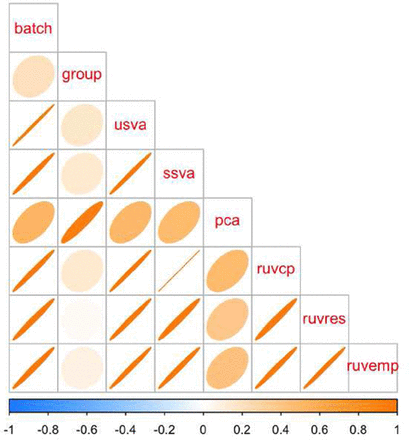
\includegraphics[width=0.45\textwidth]{leek1.png}
    \caption{Correlation between simulated batch and group variables and various batch estimates.}
  \end{figure}
\end{frame}

\begin{frame}
  \frametitle{Comparison from Leek}
  \begin{figure}
    \centering
    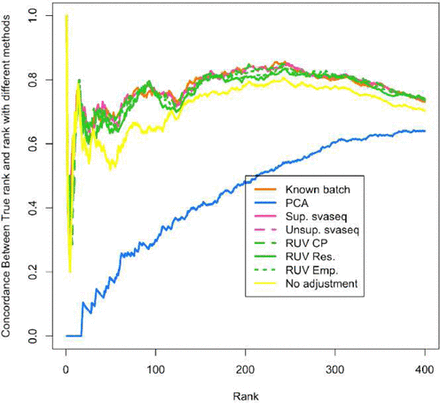
\includegraphics[width=0.45\textwidth]{leek2.png}
    \caption{Differential expression results for simulated data. A concordance at the top plot (CAT plot) shows the fraction of DE results that are concordant between the analysis with the true batch and the analyses using different batch estimates.}
  \end{figure}
\end{frame}

\begin{frame}
  \frametitle{A few other methods}
  \begin{enumerate}
  \item PEER\footcite{Stegle2012} cran R package \CRANpkg{peer}
  \item isva\footcite{Teschendorff2011} cran R package \CRANpkg{isva}
  \item RUV-4, RUV-inv, and RUV-rinv\footcite{Gagnon-Bartsch2013} cran R package \CRANpkg{ruv}
  \end{enumerate}
  These methods can also be applied to other omics-data e.g. 450k DNA methylation data
\end{frame}

\begin{frame}
  \frametitle{Background: General formulation of the problem}
  \begin{equation}
    \label{eq:general}
    Y_{n \times p} = Z_{n \times q}\alpha_{q \times p} + W_{n \times k}\beta_{k \times p} + \epsilon_{n \times p}
  \end{equation}
  \begin{itemize}
  \item $Y_{n \times p}$: observed expr. data on $n$ samples and $p$ genes
  \item $Z_{n \times q}$: $q$ known cov. including phenotype of interest
  \item $V_{n \times k}$: $k$ unobserved cov.
  \item $\alpha$, $\beta$: represent the unknown effects of the obs. and unobs. cov. on gene expr.
  \end{itemize}
\end{frame}

\begin{frame}
  \frametitle{Background: Two extremes}
  \begin{quote}
    Consider only known covariates or no covariates at all
  \end{quote}
  \begin{enumerate}
  \item Correct for known technical of biological covariates using a linear model:\\
    \begin{equation}
      \label{eq:linmod}
      Y = Z\alpha + \epsilon
    \end{equation}
    (e.g. all $\beta$'s are zero)
  \item Estimate batch effects using SVD/PC on $Y = U \Sigma V^T$ \\
    \begin{equation}
      \label{eq:svd}
      Y = W\beta + \epsilon,
    \end{equation}
    $W_{n \times k} = V_{n \times k}$: are the first $k$ principal components, the optimal $k$ needs to be determined (e.g. now all $\alpha$'s are zero)
  \end{enumerate}
\end{frame}

\begin{frame}
  \frametitle{Background: SVA}
  \begin{enumerate}
  \item[Step 1:] fit covariates of interest
    \begin{equation}
      \label{eq:sva1a}
      Y_{n \times p} = Z_{n \times 1}\alpha_{q \times p} + \epsilon_{n \times p}
    \end{equation}
    \begin{equation}
      \label{eq:sva1b}
      R_{n \times p} = Y_{n \times p} - Z_{n \times 1}\hat{\alpha}_{q \times p}
    \end{equation}
    Estimate unobserved batch effects using SVD/PC on $R = U \Sigma V^T$
  \item[Step 2:]  fit covariates of interest plus a few estimated unobserved batch effects
    \begin{equation}
      \label{eq:svafit}
      Y_{n \times p} = Z_{n \times q}\alpha_{q \times p} + W_{n \times r}\beta_{r \times p} + \epsilon_{n \times p}
    \end{equation}
    $W_{n \times k} = V_{n \times k}$: are the first $k$ principal components, the optimal $k$ is determined using permutation test on the eigenvalues\\
  \end{enumerate}
\end{frame}

\begin{frame}
  \frametitle{Background: RUV-2}
  \begin{enumerate}
  \item[Step 1:] Consider general model for $p'$ control genes
    \begin{equation}
      \label{eq:ruv21a}
      Y_{n \times p'} = Z_{n \times 1}\alpha_{q \times p'} +  + W_{n \times k}\beta_{k \times p'} + \epsilon_{n \times p'}
    \end{equation}
    the 'control gene assumption' is that $\alpha = 0$
    \begin{equation}
      \label{eq:ruv21b}
      Y_{n \times p'} = W_{n \times k}\beta_{k \times p'} + \epsilon_{n \times p'}
    \end{equation}
    $W_{n \times k} = V_{n \times k}$ SVD/PC of $Y_{n \times p'} = U \Sigma V^T$
  \item[Step 2:]  fit covariates of interest plus a few estimated unobserved batch effects
    \begin{equation}
      \label{eq:ruvfit}
      Y_{n \times p} = Z_{n \times q}\alpha_{q \times p} + W_{n \times k}\beta_{k \times p} + \epsilon_{n \times p}
    \end{equation}
    the optimal $k$ needs to be determined
  \end{enumerate}
  if $\alpha \neq 0$ for some covariates use the SVD of $Y - YZ(Z^TZ)^{-1}Z^T$ again only on the control genes
\end{frame}

\begin{frame}
  \frametitle{CATE}
\end{frame}


\begin{frame}
  \frametitle{Background: RUV-4, RUV-inv, and RUV-rinv}
  \begin{enumerate}
  \item[RUV-4:] a hybrid between RUV-2 and SVA
  \item[RUV-inv:] includes selection of the number of unobserved batches with a novel method for estimation of the variance $\cdots$
  \item[RUV-rinv:] rigde regression $\cdots$
  \end{enumerate}
\end{frame}

\begin{frame}
  \frametitle{Background: isva}
  i.s.o. using linear uncorrelated eigenvectors in the SVA method estimate statistically independent variables using independent component analysis
\end{frame}

\begin{frame}
  \frametitle{Background: PEER}
  similar to SVA estimates unobserved covariates but uses empirical Bayesian statistics
\end{frame}

\begin{frame}
  \frametitle{Relation to other methods: LMM}
\end{frame}

\end{document}
